\documentclass{article}
\usepackage{graphicx}
\usepackage{titling}  % For custom title page
\usepackage{circuitikz}
\usepackage{amsmath}
\usepackage{amssymb}
\usepackage{booktabs,tabu}
\usepackage{float}

\title{Experiment 1: Basic Filter Design}
\author{Samyak Sheersh}
\date{06 August 2024}
\newcommand{\subtitle}[1]{%
  \posttitle{%
    \par\end{table}
    \begin{center}\large#1\end{center}
    \vskip0.5em}%
}

\begin{document}

% Custom title page
\begin{titlepage}
    \centering
    
\includegraphics[width=0.2\textwidth]{KGP_logo.png}\par\vspace{1cm}
    {\scshape\LARGE Department of Electronics and Electrical Communication Engineering, IIT Kharagpur\par}
    \vspace{1cm}
    {\huge\bfseries Experiment 2:  Low Pass Filters and Windowing\par}
    \vspace{1.5cm}
    {\Large\itshape Samyak Sheersh\par}
    \vfill
    % Identifying information at the bottom
    {\large Roll Number: 22EC30045\par}
    {\large Group Number: 24\par}
    \vfill
    {\large 22 August 2024\par}
\end{titlepage}

\section{Tasks}
\begin{enumerate}
\item Designing several Finite Impulse Response (FIR) Filters and observing their frequency responses.
\item Studying the frequency responses of the same filters to noiseless and noisy inputs.
\end{enumerate}

\section{Procedure and Results}
\subsection{Task 1.1}
We pass a sinusoidal input through various windowing functions, the time domain functions of whom are given as follows: \\\\
    Rectangular window: $w(n) = 1 $ \\
    Triangular window : $w(n) = 1 - 2\dfrac{(n - \frac{N - 1}{2})}{N - 1}$ \\
    Hanning window : $w(n) = 0.5 - 0.5cos(2\pi{\dfrac{n}{N - 1}})$ \\
    Hamming window : $w(n) = 0.54 - 0.46cos(2\pi{\dfrac{n}{N - 1}})1$ \\
    Blackman window : $w(n) = 0.42 - 0.5cos(2\pi{\dfrac{n}{N - 1}}) + 0.08cos(4\pi{\dfrac{n}{N - 1}})$\\\\
Note : n runs from 0 to N - 1, and the filters output zero for all other n. The impulse response of the filters is obtained by taking the convolution of the window function with that of a low pass filter in the time domain.
\\
We wish to note the transition width of of the main lobe, the peak of the first side lobe and the maximum stop-band attenuation for all windows, at N = 8, 64 and 512.
\\
The cutoff frequency for the filters $(f_c)$ is set at $2kHz$, and the sampling frequency is fixed at 12kHz.
\clearpage
\begin{table}
\centering
\caption{Simulated values for Rectangular Window.}
\begin{tabular}{||c c c c||} 
 \hline
 N & Transition Width (kHz) & First Side Lobe (dB) & Max Attenuation (dB)\\ [0.5ex] 
 \hline\hline
 8 & 2.30 & -19.4 & -45 \\ 
 64 & 0.25 & -20.9 & -51 \\
 512 & 0.02 & -21.1 & -70 \\   
 \hline
\end{tabular}
\end{table}

\begin{table}
\centering
\caption{Simulated values for Triangular Window.}
\begin{tabular}{||c c c c||} 
 \hline
 N & Transition Width (kHz) & First Side Lobe (dB) & Max Attenuation (dB)\\ [0.5ex] 
 \hline\hline
 8 & 2.63 & -20.9 & -26 \\ 
 64 & 0.28 & -20.6 & -37 \\
 512 & 0.05 & -20.7 & -60 \\   
 \hline
\end{tabular}
\end{table}

\begin{table}
\centering
\caption{Simulated values for Hanning Window.}
\begin{tabular}{||c c c c||} 
 \hline
 N & Transition Width (kHz) & First Side Lobe (dB) & Max Attenuation (dB)\\ [0.5ex] 
 \hline\hline
 8 & 4.45 & -44.1 & -55 \\ 
 64 & 0.59 & -44.1 & -137 \\
 512 & 0.09 & -44.1 & -194 \\   
 \hline
\end{tabular}
\end{table}

\begin{table}
\centering
\caption{Simulated values for Hamming Window.}
\begin{tabular}{||c c c c||} 
 \hline
 N & Transition Width (kHz) & First Side Lobe (dB) & Max Attenuation (dB)\\ [0.5ex] 
 \hline\hline
 8 & 4.46 & -48.3 & -60 \\ 
 64 & 0.59 & -52.3 & -71 \\
 512 & 0.09 & -55.0 & -93 \\   
 \hline
\end{tabular}
\end{table}
\begin{table}
\centering
\caption{Simulated values for Blackman Window.}
\begin{tabular}{||c c c c||} 
 \hline
 N & Transition Width (kHz) & First Side Lobe (dB) & Max Attenuation (dB)\\ [0.5ex] 
 \hline\hline
 8 & 4.98 & -53.0 & -54 \\ 
 64 & 0.92 & -75.5 & -147 \\
 512 & 0.12 & -75.6 & -201 \\   
 \hline
\end{tabular}
\end{table}

\begin{figure}[H]
    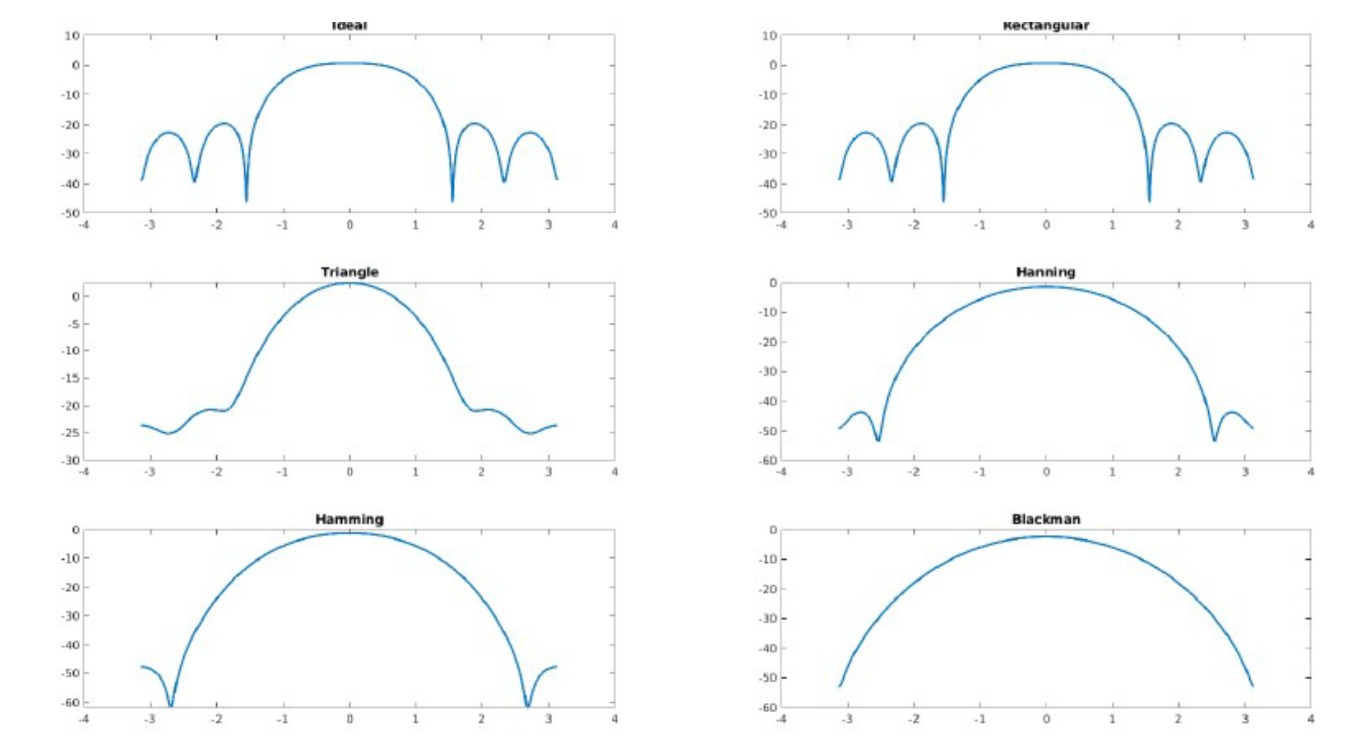
\includegraphics[width=\textwidth]
    {N=8.jpg}
    \caption{Frequency Response of Filters for N = 8.}
    \end{figure}

\begin{figure}[H]
    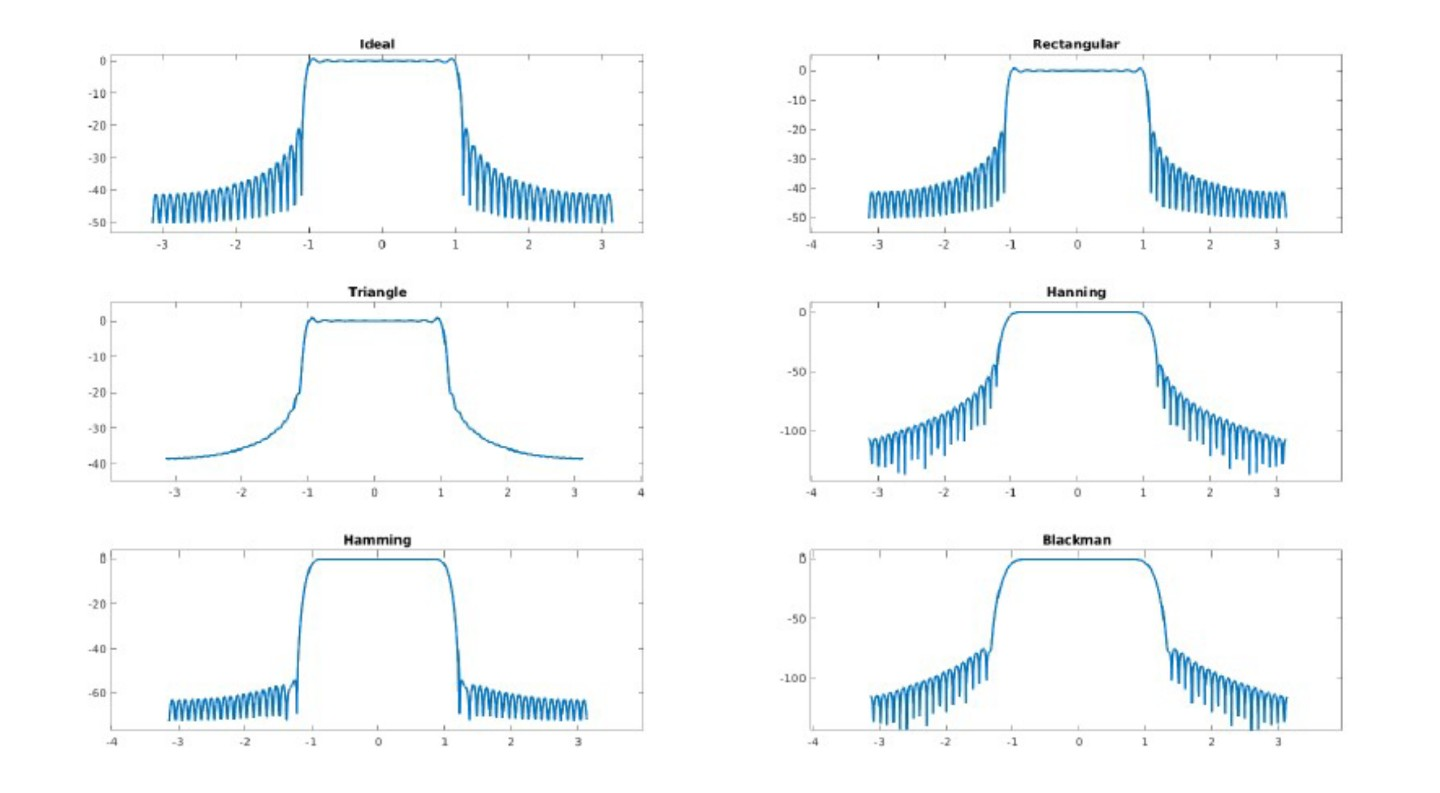
\includegraphics[width=\textwidth]
    {N=64.jpg}
    \caption{Frequency Response of Filters for N = 64.}
    \end{figure}

    \begin{figure}[H]
    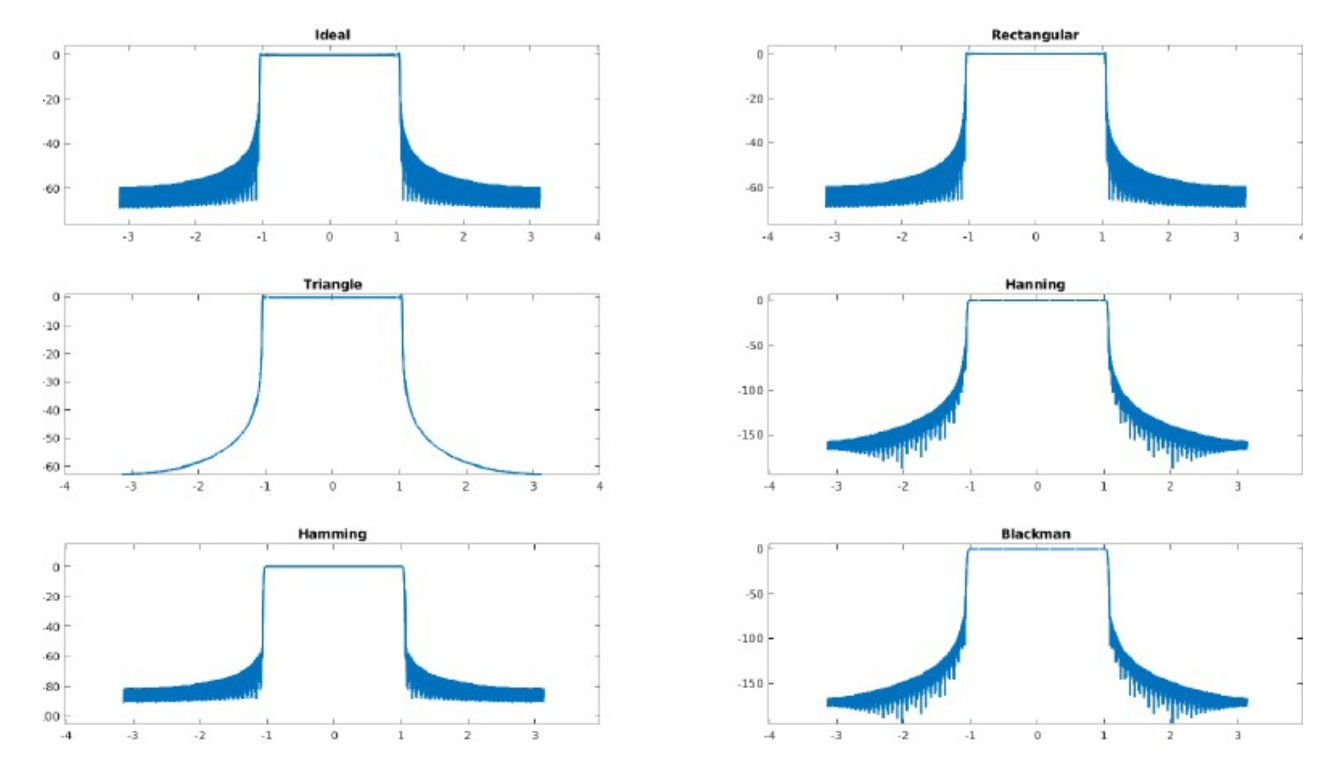
\includegraphics[width=\textwidth]
    {N=512.jpg}
    \caption{Frequency Response of Filters for N = 512.}
    \end{figure}

\subsection{Task 1.2}
We now generate a signal comprised of two frequencies, one within the pass band of the earlier filter and one outside of it. Our resultant input signal now becomes,
\begin{equation}
    x(t) = sin(2{\pi}f_{L}t) + sin(2{\pi}f_{H}t)
\end{equation}
We take $f_{L} = 1kHz$, and $f_{H} = 3kHz$ respectively. We then calculate the SNR (Signal to Noise Ratio) for various values of N for each filter.

\begin{table}
\centering
\caption{SNR values of all filters across different N.}
\begin{tabular}{||c c c c c c||} 
 \hline
 N & Rectangular (kHz) & Triangular & Hanning & Hamming & Blackman\\ [0.5ex] 
 \hline\hline
 8 & 13.6 & 15.5 & 8.6 & 9.3 & 7.4 \\
 64 & 13.9 & 14.3 & 14.0 & 14.0 & 14.0 \\
 512 & 13.9 & 13.9 & 13.9 & 13.9 & 13.9 \\ 
 \hline
\end{tabular}
\end{table}

\begin{figure}[H]
    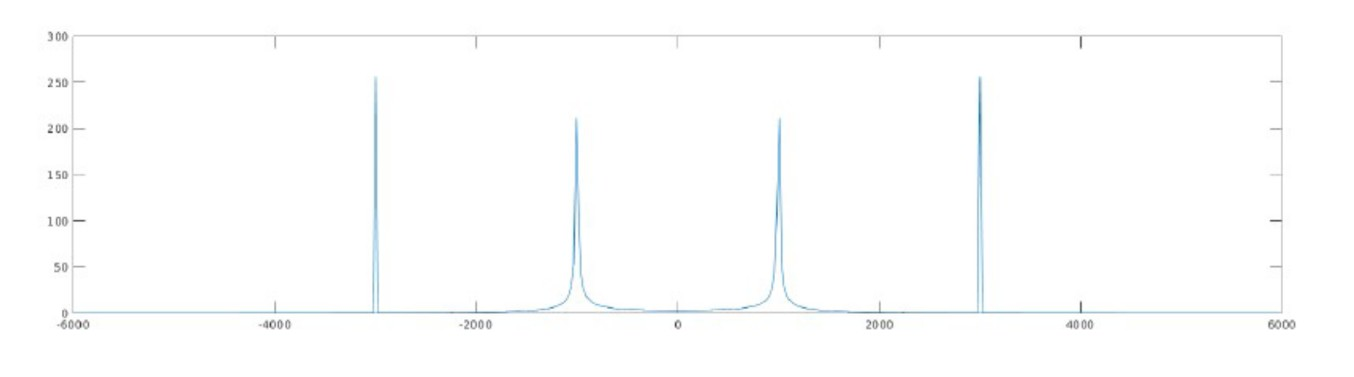
\includegraphics[width=\textwidth]
    {input_wave.jpg}
    \caption{Input without noise in frequency domain.}
    \end{figure}
    \begin{figure}[H]
    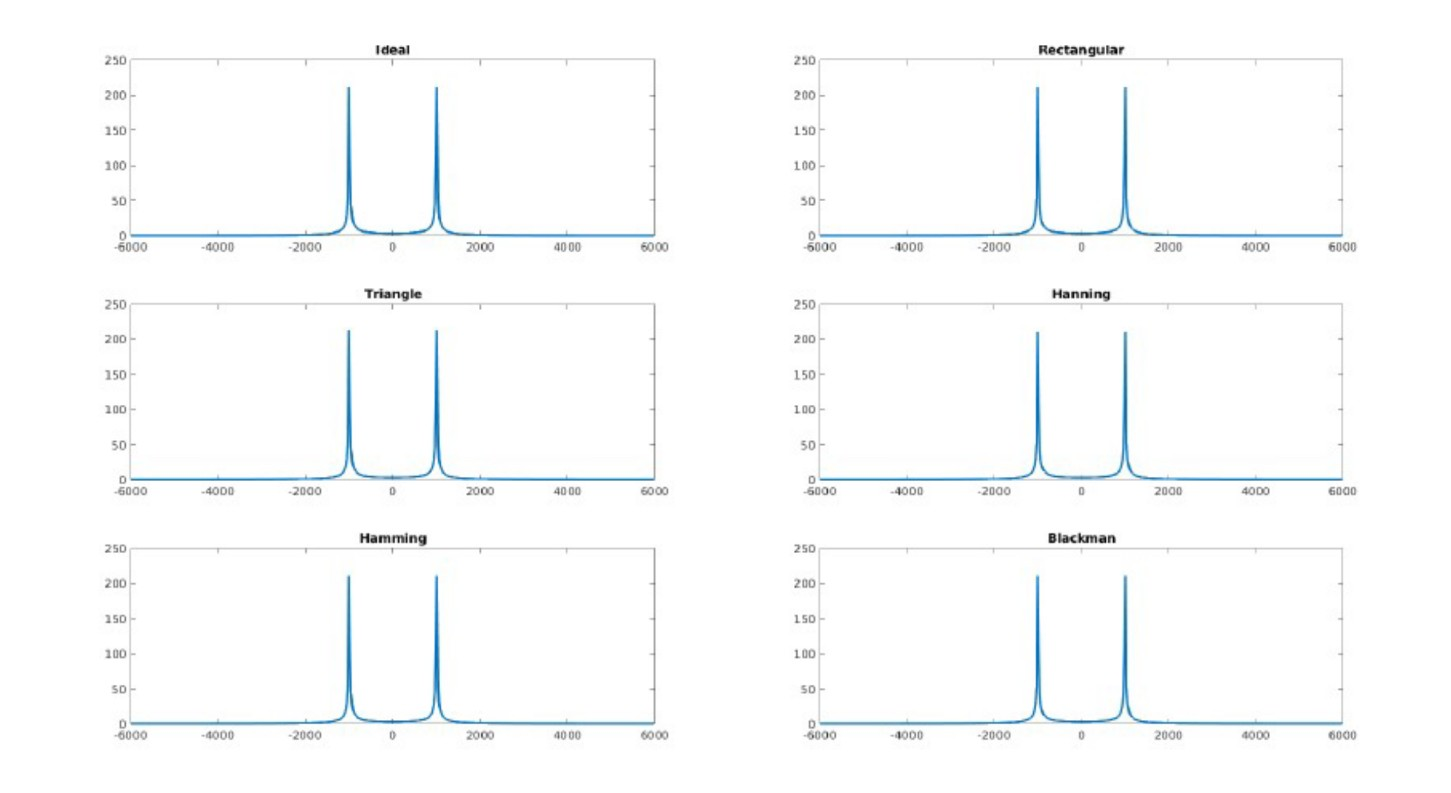
\includegraphics[width=\textwidth]
    {pure_response.jpg}
    \caption{Frequency Response of Filters to Noiseless Signal.}
    \end{figure}
    \begin{figure}[H]
    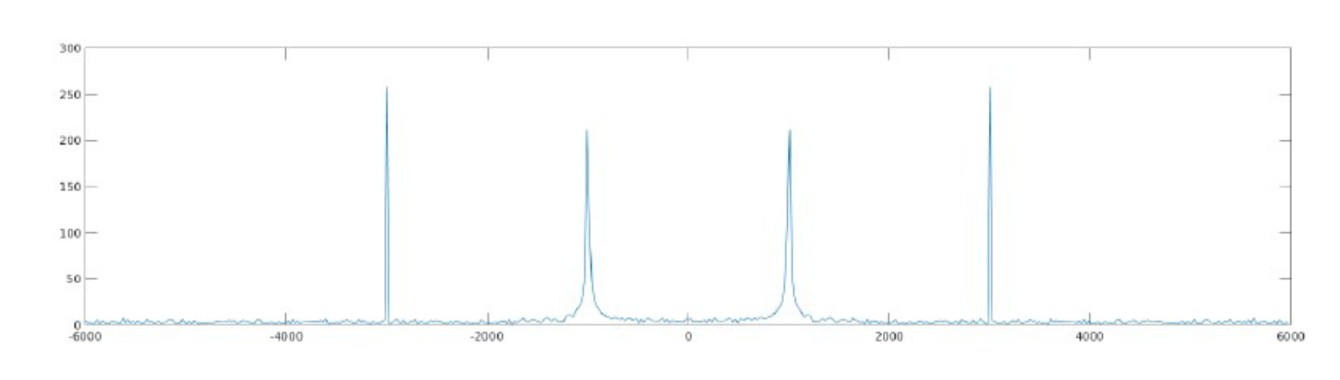
\includegraphics[width=\textwidth]
    {noisy_input.jpg}
    \caption{Input with noise in frequency domain.}
    \end{figure}
    \begin{figure}[H]
    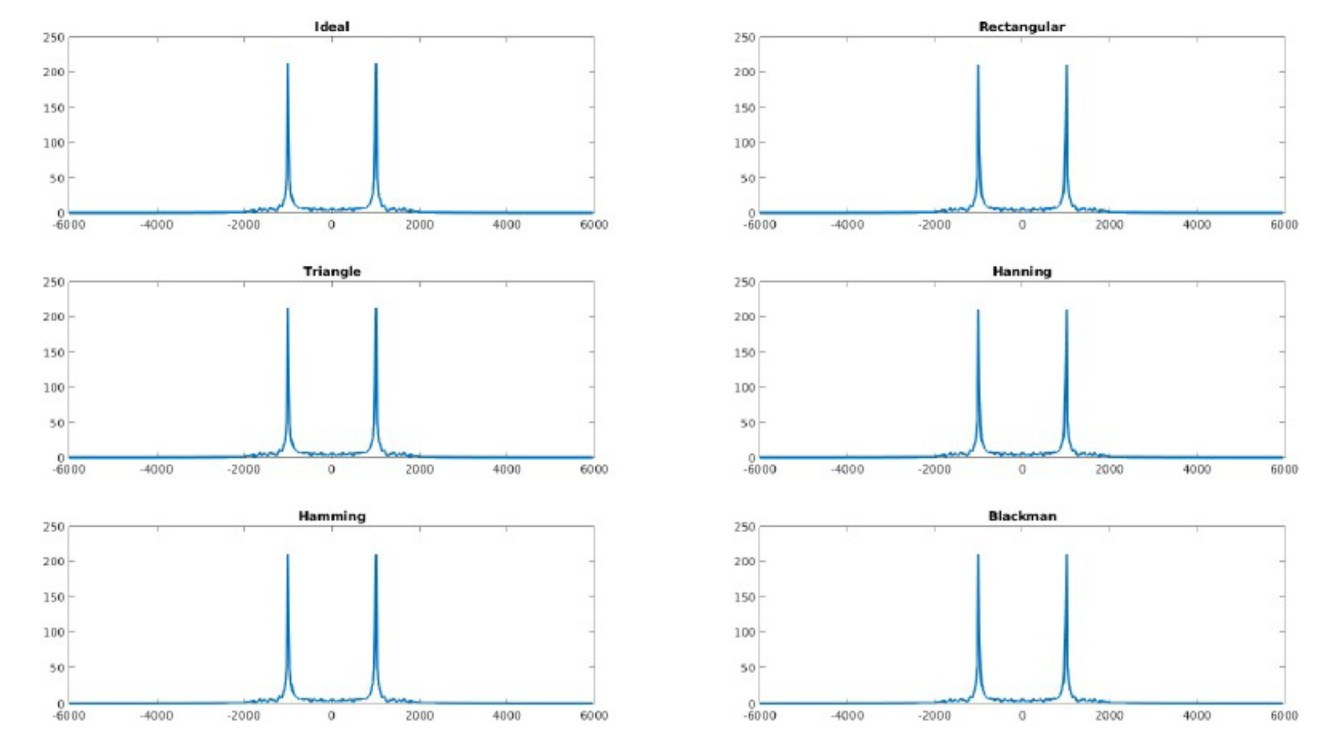
\includegraphics[width=\textwidth]
    {noisy_response.jpg}
    \caption{Frequency Response of Filters to Noisy Signal.}
    \end{figure}

\section{Discussions}
\subsection{Samyak Sheersh, 22EC30045}
\begin{enumerate}
    \item We learned about FIR filter design in this experiment, since an ideal LPF would be bandlimited an thus an a time representation which is infinite, we need to create real filters which will be time limited
    \item To create an FIR filter, we would need to truncate the sinc(t) representation of the ideal low-pass filter, which would result in non-idealities in the frequency domain, in the form of ripples due to the Gibbs' Phenomenon
    \item  Windowing is basically taking a finite window of the sinc function, and gradually reducing it within the window, similar to emulating the entire sinc function but inside the window
    \item At larger values of N, we got a flat pass band and lesser energy stored in the ripples, thus indicating a closer and more efficient approximation. The transition width remained the same though.
    \item For larger values of N, we also saw that the SNR generally got higher, although the increase wasn't too extreme
\end{enumerate}
\end{document}
